\documentclass[12pt,fleqn]{article}\usepackage{../common}

\begin{document}
Google Nasil Isler? 

Google arama motoruna bir kelime yazdigimizda geri gelen sonuclar nasil
kararlastirilir? Ilk akla gelen yontem tabii ki Web'deki tum sayfalarin
(milyarlarca sayfa) sayfalar uzerindeki kelimelerin o sayfa ile
iliskilendirilmesi ve arama yapilinca kelimeye gore sayfa geri
getirilmesi. Mesela alttaki ornekte ``book (kitap)'' yazinca geriye 1.,
2. ve 5. sayfalar geri gelecek. Fakat hangi sirada? Bu sayfalardan hangisi
digerlerinden daha onemli?

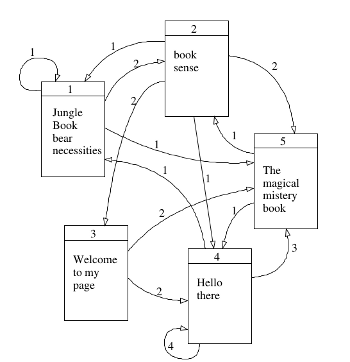
\includegraphics[height=9cm]{pg2.png}

Google'in arama motorlarina getirdigi en buyuk yeniliklerden biri PageRank
algoritmasidir. Bu algoritmanin temelinde daha fazla referans edilen
sayfalar daha ustte cikmasi yatar. Hatta o referans eden sayfalarin
kendilerine daha fazla referans var ise bu etki ta en sondaki sayfaya kadar
yansitilir, hatta bu zincir bastan sona her seviyede hesaplanabilir. Peki bu
nasil gerceklestirilir?

PageRank Web sayfalarini bir Markov Zincir olarak gorur. Markov Zincirleri
seri halindeki $X_n, n=0,1,2,..$ rasgele degiskenini modeller ve bu
degiskenler belli sayidaki konumlarin birinde olabilirler. Mesela konumlari
bir dogal sayi ile ilintilendirirsek $X_n = i$ olabilir ki $i=\{0,1,..\}$
diye kabul edelim. 

Markov Zincirlerinde (MZ) $i$ konumundan $j$ konumuna gecis olasiligini,
$P_{ij}$, biliriz ve bu $P(X_{n+1} = j | X_{n} = i)$ olarak acilabilir. Acilimdan  
gorulecegi uzere bir MZ sonraki adima gecis olasiligi icin sadece
bir onceki adima bakar. Bu tur once/sonra yapisindaki iki boyutlu hal, 
cok rahat bir sekilde matrisina cevirilebilir / gosterilebilir. Onceki konum 
satirlar, sonraki konum kolonlar olarak betimlenir mesela. 

Ornek

Bir sonraki gunde yagmur yagmayacagini bir MZ olarak tasarlayalim. Bir
sonraki gunde yagmur yagmayacagini sadece bugun etkiliyor olsun. Eger bugun
yagmur yagiyorsa yarin yagmur yagmasi 0.7, eger bugun yagmiyor ise yarin
yagmasi 0.4. MZ soyle

$$ 
P =
\left[\begin{array}{cc}
0.7 & 0.3 \\
0.4 & 0.6
\end{array}\right]
 $$

Gecis olasiliklarindan bahsettigimize gore ve elimizde sinirli / belli
sayida konum var ise, bir MZ'nin her satirindaki olasiliklarin toplami
tabii ki 1'e esit olmalidir. 

MZ'lerin ilginc bir ozelligi $n$ adim sonra $i,j$ gecisinin $P^n$ hesabiyla
yapilabilmesidir. Yani $P$'yi $n$ defa kendisiyle carpip $i,j$ kordinatina 
bakarsak $n$ adim sonrasini rahatca gorebiliriz. Bunun ispatini burada
vermeyecegiz. 

Mesela ustteki ornekte, eger bugun yagmur yagiyorsa 4 gun sonra yagmur
yagma olasiligi nedir? 

\begin{minted}{python}
import numpy.linalg as lin
P = np.array([[0.7,0.3],[0.4,0.6]])
P4 = lin.matrix_power(P,4)
print P4
\end{minted}

\begin{verbatim}
[[ 0.5749  0.4251]
 [ 0.5668  0.4332]]
\end{verbatim}

Aradigimiz gecis icin kordinat 0,0'a bakiyoruz ve sonuc 0.5749. Numpy
\verb!matrix_power! bir matrisi istedigimiz kadar kendisiyle carpmamizi
sagliyor. 

\begin{minted}{python}
K = 4
  
T = [[1./4, 2./4, 0, 0, 1./4],
     [1./6, 0, 2./6, 1./6, 2./6],
     [0, 0, 0, 2./4, 2./4],
     [1./8, 0, 0, 4./8, 3./8],
     [0, 1./2, 0, 1./2, 0]]

T = np.array(T)
print T
\end{minted}

\begin{verbatim}
[[ 0.25        0.5         0.          0.          0.25      ]
 [ 0.16666667  0.          0.33333333  0.16666667  0.33333333]
 [ 0.          0.          0.          0.5         0.5       ]
 [ 0.125       0.          0.          0.5         0.375     ]
 [ 0.          0.5         0.          0.5         0.        ]]
\end{verbatim}



[1] Murphy, K., CS340: Machine Learning Lecture Notes, \url{www.ugrad.cs.ubc.ca/~cs340}

[2] Ross, S., Introduction to Probability Models, 8th Edition

\end{document}
